When considering the design space of mappings $M = A^K$ we usually consider no relationship between mappings.
For two mappings we can say if they are identical or not, or perhaps with the methods of Chapter~\ref{chap:symmetries} if they are \emph{equivalent} or not.
However, any further relationship we can't describe: can we say that two mappings are very similar, or very different?
Can we quantify the \emph{distance} between two mappings?
Intuitively, we can.
This section requires some basic concepts from the mathematic theory of (discrete) metric spaces and embeddings into real spaces.
Appendix~\ref{appendix:metric} gives an overview of the required concepts, a more thorough exposition can be found in~\cite{matouvsek}, Chapter~15 in particular.

Normally, we encode mappings as vectors $m = \left[ a_1, \ldots, a_{|V_K|} \right]$ where $a_i \in V_A$ are the \acp{PE} where task $i$ is mapped.
If we interpret these vectors as being (real) vectors in $\mathbb{R}^{|V_K|}$, we can endow them with a vector distance, like the Euclidean distance $d_\text{Euclidean}(v,w) = \sqrt{\sum_i (v_i - w_i)^2}$.
This can be generalized to other $p$-norms, as $d_{L_p}(v,w) = \sum_i ((|v_i-w_i|)^p)^{1/p}$, which is a norm for $p \geq 1$.
For $p = 1$, this norm is also known as the Mathattan distance, in allusion to the distance between buildings in a regular mesh like the streets of Manhattan.
We can endow the space of mappings with a metric also by using the Hamming metric, which counts only the number of differing entries in the vector.
However, none of these metrics are ideal for the mapping space, as we will now explain.

\begin{figure}[h]
	\centering
   \resizebox{0.85\textwidth}{!}{
	   \begin{tikzpicture}
	   \begin{scope}[name prefix=m1-, scale=0.25,every node/.append style={scale=0.25},]
%little cores
\node (pe1) at ({-1.5},{4}) [draw,minimum width=2.5cm,align=center,minimum height=2cm, fill=green!30] {\huge PE$_1$};
\node (L1-pe1) at (-1.5,2.5) [draw,minimum width=2.5cm,align=center,minimum height=1.5cm, fill=blue!30] {\huge L1\$};
\node (pe2) at (-1.5+3,4) [draw,minimum width=2.5cm,align=center,minimum height=2cm, fill=green!30] {\huge PE$_2$};
\node (L1-pe2) at (-1.5+3,2.5) [draw,minimum width=2.5cm,align=center,minimum height=1.5cm, fill=blue!30] {\huge L1\$};
\node (pe3) at (-1.5,4+4) [draw,minimum width=2.5cm,align=center,minimum height=2cm, fill=green!30] {\huge PE$_3$};
\node (L1-pe3) at (-1.5,2.5+4) [draw,minimum width=2.5cm,align=center,minimum height=1.5cm, fill=blue!30] {\huge L1\$};
\node (pe4) at (-1.5+3,4+4) [draw,minimum width=2.5cm,align=center,minimum height=2cm, fill=green!30] {\huge PE$_4$};
\node (L1-pe4) at (-1.5+3,2.5+4) [draw,minimum width=2.5cm,align=center,minimum height=1.5cm, fill=blue!30] {\huge L1\$};

%big cores
\node (pe5) at ({6.5-1.5},{4}) [draw,minimum width=2.5cm,align=center,minimum height=2cm, fill=green!60] {\huge PE$_5$};
\node (L1-pe5) at (6.5-1.5,2.5) [draw,minimum width=2.5cm,align=center,minimum height=1.5cm, fill=blue!30] {\huge L1\$};
\node (pe6) at (6.5-1.5+3,4) [draw,minimum width=2.5cm,align=center,minimum height=2cm, fill=green!60] {\huge PE$_6$};
\node (L1-pe6) at (6.5-1.5+3,2.5) [draw,minimum width=2.5cm,align=center,minimum height=1.5cm, fill=blue!30] {\huge L1\$};
\node (pe7) at (6.5-1.5,4+4) [draw,minimum width=2.5cm,align=center,minimum height=2cm, fill=green!60] {\huge PE$_7$};
\node (L1-pe7) at (6.5-1.5,2.5+4) [draw,minimum width=2.5cm,align=center,minimum height=1.5cm, fill=blue!30] {\huge L1\$};
\node (pe8) at (6.5-1.5+3,4+4) [draw,minimum width=2.5cm,align=center,minimum height=2cm, fill=green!60] {\huge PE$_8$};
\node (L1-pe8) at (6.5-1.5+3,2.5+4) [draw,minimum width=2.5cm,align=center,minimum height=1.5cm, fill=blue!30] {\huge L1\$};


\node (L2-little) at (0,0) [draw,minimum width=6cm,align=center,minimum height=1.5cm, fill=blue!55] {\huge L2\$};
\node (L2-big) at (6.5,0) [draw,minimum width=6cm,align=center,minimum height=1.5cm, fill=blue!55] {\huge L2\$};
\node (DRAM) at (3.25,-2.5) [minimum width=12.5cm,align=center,minimum height=2cm, fill=blue!85] {\huge DRAM};
\node[ellipse,fill=red!60] (t1) at (pe2) {\Huge t$_1$};
\node[ellipse,fill=red!60] (t2) at (pe1) {\Huge t$_2$};
\draw (t1) edge[-{latex},line width=0.2mm, color=red!80] (t2);
\end{scope}

\begin{scope}[xshift=125,name prefix=m2-, scale=0.25,every node/.append style={scale=0.25},]
%little cores
\node (pe1) at ({-1.5},{4}) [draw,minimum width=2.5cm,align=center,minimum height=2cm, fill=green!30] {\huge PE$_1$};
\node (L1-pe1) at (-1.5,2.5) [draw,minimum width=2.5cm,align=center,minimum height=1.5cm, fill=blue!30] {\huge L1\$};
\node (pe2) at (-1.5+3,4) [draw,minimum width=2.5cm,align=center,minimum height=2cm, fill=green!30] {\huge PE$_2$};
\node (L1-pe2) at (-1.5+3,2.5) [draw,minimum width=2.5cm,align=center,minimum height=1.5cm, fill=blue!30] {\huge L1\$};
\node (pe3) at (-1.5,4+4) [draw,minimum width=2.5cm,align=center,minimum height=2cm, fill=green!30] {\huge PE$_3$};
\node (L1-pe3) at (-1.5,2.5+4) [draw,minimum width=2.5cm,align=center,minimum height=1.5cm, fill=blue!30] {\huge L1\$};
\node (pe4) at (-1.5+3,4+4) [draw,minimum width=2.5cm,align=center,minimum height=2cm, fill=green!30] {\huge PE$_4$};
\node (L1-pe4) at (-1.5+3,2.5+4) [draw,minimum width=2.5cm,align=center,minimum height=1.5cm, fill=blue!30] {\huge L1\$};

%big cores
\node (pe5) at ({6.5-1.5},{4}) [draw,minimum width=2.5cm,align=center,minimum height=2cm, fill=green!60] {\huge PE$_5$};
\node (L1-pe5) at (6.5-1.5,2.5) [draw,minimum width=2.5cm,align=center,minimum height=1.5cm, fill=blue!30] {\huge L1\$};
\node (pe6) at (6.5-1.5+3,4) [draw,minimum width=2.5cm,align=center,minimum height=2cm, fill=green!60] {\huge PE$_6$};
\node (L1-pe6) at (6.5-1.5+3,2.5) [draw,minimum width=2.5cm,align=center,minimum height=1.5cm, fill=blue!30] {\huge L1\$};
\node (pe7) at (6.5-1.5,4+4) [draw,minimum width=2.5cm,align=center,minimum height=2cm, fill=green!60] {\huge PE$_7$};
\node (L1-pe7) at (6.5-1.5,2.5+4) [draw,minimum width=2.5cm,align=center,minimum height=1.5cm, fill=blue!30] {\huge L1\$};
\node (pe8) at (6.5-1.5+3,4+4) [draw,minimum width=2.5cm,align=center,minimum height=2cm, fill=green!60] {\huge PE$_8$};
\node (L1-pe8) at (6.5-1.5+3,2.5+4) [draw,minimum width=2.5cm,align=center,minimum height=1.5cm, fill=blue!30] {\huge L1\$};


\node (L2-little) at (0,0) [draw,minimum width=6cm,align=center,minimum height=1.5cm, fill=blue!55] {\huge L2\$};
\node (L2-big) at (6.5,0) [draw,minimum width=6cm,align=center,minimum height=1.5cm, fill=blue!55] {\huge L2\$};
\node (DRAM) at (3.25,-2.5) [minimum width=12.5cm,align=center,minimum height=2cm, fill=blue!85] {\huge DRAM};
\node[ellipse,fill=red!60] (t1) at (pe2) {\Huge t$_1$};
\node[ellipse,fill=red!60] (t2) at (pe4) {\Huge t$_2$};
\draw (t1) edge[-{latex},line width=0.2mm, color=red!80] (t2);
\end{scope}

\begin{scope}[xshift=250,name prefix=m3-, scale=0.25,every node/.append style={scale=0.25},]
%little cores
\node (pe1) at ({-1.5},{4}) [draw,minimum width=2.5cm,align=center,minimum height=2cm, fill=green!30] {\huge PE$_1$};
\node (L1-pe1) at (-1.5,2.5) [draw,minimum width=2.5cm,align=center,minimum height=1.5cm, fill=blue!30] {\huge L1\$};
\node (pe2) at (-1.5+3,4) [draw,minimum width=2.5cm,align=center,minimum height=2cm, fill=green!30] {\huge PE$_2$};
\node (L1-pe2) at (-1.5+3,2.5) [draw,minimum width=2.5cm,align=center,minimum height=1.5cm, fill=blue!30] {\huge L1\$};
\node (pe3) at (-1.5,4+4) [draw,minimum width=2.5cm,align=center,minimum height=2cm, fill=green!30] {\huge PE$_3$};
\node (L1-pe3) at (-1.5,2.5+4) [draw,minimum width=2.5cm,align=center,minimum height=1.5cm, fill=blue!30] {\huge L1\$};
\node (pe4) at (-1.5+3,4+4) [draw,minimum width=2.5cm,align=center,minimum height=2cm, fill=green!30] {\huge PE$_4$};
\node (L1-pe4) at (-1.5+3,2.5+4) [draw,minimum width=2.5cm,align=center,minimum height=1.5cm, fill=blue!30] {\huge L1\$};

%big cores
\node (pe5) at ({6.5-1.5},{4}) [draw,minimum width=2.5cm,align=center,minimum height=2cm, fill=green!60] {\huge PE$_5$};
\node (L1-pe5) at (6.5-1.5,2.5) [draw,minimum width=2.5cm,align=center,minimum height=1.5cm, fill=blue!30] {\huge L1\$};
\node (pe6) at (6.5-1.5+3,4) [draw,minimum width=2.5cm,align=center,minimum height=2cm, fill=green!60] {\huge PE$_6$};
\node (L1-pe6) at (6.5-1.5+3,2.5) [draw,minimum width=2.5cm,align=center,minimum height=1.5cm, fill=blue!30] {\huge L1\$};
\node (pe7) at (6.5-1.5,4+4) [draw,minimum width=2.5cm,align=center,minimum height=2cm, fill=green!60] {\huge PE$_7$};
\node (L1-pe7) at (6.5-1.5,2.5+4) [draw,minimum width=2.5cm,align=center,minimum height=1.5cm, fill=blue!30] {\huge L1\$};
\node (pe8) at (6.5-1.5+3,4+4) [draw,minimum width=2.5cm,align=center,minimum height=2cm, fill=green!60] {\huge PE$_8$};
\node (L1-pe8) at (6.5-1.5+3,2.5+4) [draw,minimum width=2.5cm,align=center,minimum height=1.5cm, fill=blue!30] {\huge L1\$};


\node (L2-little) at (0,0) [draw,minimum width=6cm,align=center,minimum height=1.5cm, fill=blue!55] {\huge L2\$};
\node (L2-big) at (6.5,0) [draw,minimum width=6cm,align=center,minimum height=1.5cm, fill=blue!55] {\huge L2\$};
\node (DRAM) at (3.25,-2.5) [minimum width=12.5cm,align=center,minimum height=2cm, fill=blue!85] {\huge DRAM};
\node[ellipse,fill=red!60] (t1) at (pe2) {\Huge t$_1$};
\node[ellipse,fill=red!60] (t2) at (pe5) {\Huge t$_2$};
\draw (t1) edge[-{latex},line width=0.2mm, color=red!80] (t2);
\end{scope}


   
\draw [decorate,decoration={brace,amplitude=5pt,mirror,raise=8ex}]
(m1-L2-little.south) -- (m2-L2-little.south) node[midway,yshift=-8em]{dist $ = \sqrt{(4 - 1)^2} = 3$ };

\draw [decorate,decoration={brace,amplitude=5pt,mirror,raise=8ex}]
(m2-L2-big.south) -- (m3-L2-big.south) node[midway,yshift=-8em]{dist $ = \sqrt{(4 - 5)^2} = 1$ };
	   \end{tikzpicture}
	   }
	\caption{An intuitive example of distance between mappings.}
	\label{fig:intuition_metric}
\end{figure}

Consider the example in Figure~\ref{fig:intuition_metric}. 
It shows three mappings 
\begin{align*}
	m_1: & & t_1 \mapsto \PE_2, & t_2 \mapsto \PE_1; \\ 
	m_2: & & t_1 \mapsto \PE_2, & t_2 \mapsto \PE_4; \\ 
	m_3: & & t_1 \mapsto \PE_2, & t_2 \mapsto \PE_5. \\ 
\end{align*}
We would normally write these mappings as vectors, $m_1 = \left[ 2, 1 \right], m_2 = \left[ 2, 4 \right]$ and $m_2 = \left[ 2, 5 \right].$
If we calculate the standard (Euclidean) distance of these vectors, then $m_2$ is farther away from $m_1$ than from $m_3$.
However, we know that communication between $\PE_1$ and $\PE_4$ is much faster than between $\PE_4$ and $\PE_5$. 
The Euclidean distance in the mapping space does not reflect the structure of the communication subsystem.

\subsection{Architectures}

In the example illustrated in Figure~\ref{fig:intuition_metric} we saw intuitively how mappings can be more or less similar.
This intuitive notion clearly depends on the underlying architecture.
It is the hardware architecture that determines the cost of communicating data between processes.
In order to endow the space of mappings with a metric space structure, we should first do so with the architecture.

We can use the intuition behind the example to define a metric that takes latency into account this way $M$~\cite{goens_mcsoc18}.
The fundamental observation here is that in a multicore architecture, communication between different \acp{PE} takes different amounts of time.
There are multiple problems with using the communication time between \acp{PE} directly as a distance between \acp{PE}.
Firstly, communication times depend on multiple factors: the latency and bandwidth of the communication resources used, the amount of data being sent, the (software) communication protocol, clock synchronization between hardware resources like the \acp{PE} and buses, arbitration or other contention issues, etc.
Of course, we can model these to various degrees.
However, the distance between \acp{PE} needs to be a fixed number and not a function of all these factors.
As an approximation, however, we can use the expected latency for a package of a standardized size (e.g. $8$ bytes).
As an expected value, this is a fixed number, but through its statistical nature it can include as much complexity in the model as required\footnote{If communication in the architecture is asymmetric, this will not define a metric. We can average the communication from $p$ to $q$ and from $q$ to $p$ to fix this, but we should probably consider this case separately.}.

The second issue we run into when using communication times for defining a distance is that, by definition, the distance between a point and itself has to be $0$, but usually a PE has to communicate with itself using an $L1$ cache, scratchpad memory or similar, which has a small but non-zero latency. In this sense, the expected communication latency between cores is \textbf{not} a metric space distance, but it approximates one well. We propose thus to ignore this latency and set the distance to 0, to obtain the mathematical metric space structure. 

Finally, this metric space structure depends strongly on the unit used to measure latency (e.g. cycles, milliseconds, etc), as well as on the absolute speed of the communication sub-architecture.
Since the goal of exposing this structure is to leverage it for algorithmic decisions like finding good mappings, it is useful to have comparable distances between different architectures.
For this, we propose to norm the metric distance function such that the average distance between \acp{PE} is $1$.

Put together, these principles yield the following definition:
\begin{defn}[Architecture Metric Space]
	\label{defn:metric_simple}
Let $A = (P,E)$ be an architecture graph and $\operatorname{lat} : P -> P$ be the expected latency between PEs.
Then we set
\begin{align}
  d_A : P \times P, (p,q) \mapsto \left\{
      \begin{array}{rr}
        \operatorname{lat}(p,q), & \text{ if } p \neq q \\
        0, & \text{otherwise}
      \end{array} \right.
      \end{align}
\end{defn}
\begin{rem}
For an architecture graph $A = (P,E)$, the tuple $(P,d_A)$ is a metric space.
\begin{bew}
Obviously $d_A(p,p) = 0$ for all $p \in P$, by definition, and $d_A(p,q) > 0$ for $p \neq q$ since the expected latency between PEs is always greater than 0.
For $p,q,r \in P$ we have $d_A(p,q) + d_A(q,r) \geq d_A(p,r)$ since the expected latency of moving data from $p$ to $q$ and then to $r$ will always be at least as much as moving it from $p$ to $r$ directly.
\end{bew}
\end{rem}


In this way we endow $M$ with a discrete metric space structure, with a metric that reflects the memory subsystem of the architecture, or more generally, its communication.
While this allows for a simple and powerful mathematical definition, a metric space structure can be inefficient for calculations.
To cope with this, we will also discuss low-distortion embeddings and show how we can find them for the metric spaces introduced.
Appendix~\ref{appendix:metric} reviews the basic notions of metric spaces, as well as more advanced concepts needed to introduce and find the more computationally efficient low-distortion embeddings.

Unfortunately, this metric also has some issues.
In particular, it does not distinguish between core types on heterogeneous systems.
To fix this, we propose an alternative metric space structure on $M$, by adding extra dimensions for the communication and the computation.
This is fundamentally very similar to adding channels in the mapping vectors.
We thus define a metric on the channels, based on the metric defined by Definition~\ref{def:metric_simple}.
The distance between two channels $c,c' \in E_A$ is defined as $|\operatorname{lat}(c_1) - lat(c_2)|$ for the communication channel between the cores.
We then do a similar concept for the cores, and take relative values of the expected runtime. 
Disregarding the \ac{ISA} or micro-architecture, we can use the frequencies as a first estimation, which is what we do here.
Obviously the frequency is not the best estimation of the expected differences in execution times between \acp{PE}, but we restrict our consideration to this for the scope of this thesis.
Future work should focus on finding better metrics for the mapping space.

This definition will not produce a metric, since distinct cores which are equivalent will have a distance of $0$, and similarly equivalent channels. 
To deal with this, we add a minimal distance between the cores (e.g. $0.1$ times the distance between the next two core types).

\subsubsection{Application distances}

To go from $A$ to $M$, we can use the same principle as the $L_p$ norms and define $d(m,m') = (\sum_i d(m_i,m'_i)^p)^{1/p}$, which can immediately be checked to be a metric on $M$.
This way we can consider, as a metric space (embedding), the structure of $A$ to be
 \begin{align} \label{eqn:orthogonal_sum} \underbrace{M \bot \ldots \bot M}_{ \times |V_K|}. \end{align} 

There are multiple issues with this as well. 
A very crucial problem with it is that this does not consider the dependencies between tasks in the application graph $A$, nor does it consider how multiple tasks might be more or less relevant.
Many methods can be considered to account for this fact, like having factors for the dimensions of the copies of $M$ in the orthogonal sum.
However, we omit evaluating multiple such metrics to limit the scope of this thesis.

\begin{figure}[h]
	\centering
   \resizebox{0.85\textwidth}{!}{
	   \begin{tikzpicture}
	   \begin{scope}[name prefix=m1-, scale=0.25,every node/.append style={scale=0.25},]
%little cores
\node (pe1) at ({-1.5},{4}) [draw,minimum width=2.5cm,align=center,minimum height=2cm, fill=green!30] {\huge PE$_1$};
\node (L1-pe1) at (-1.5,2.5) [draw,minimum width=2.5cm,align=center,minimum height=1.5cm, fill=blue!30] {\huge L1\$};
\node (pe2) at (-1.5+3,4) [draw,minimum width=2.5cm,align=center,minimum height=2cm, fill=green!30] {\huge PE$_2$};
\node (L1-pe2) at (-1.5+3,2.5) [draw,minimum width=2.5cm,align=center,minimum height=1.5cm, fill=blue!30] {\huge L1\$};
\node (pe3) at (-1.5,4+4) [draw,minimum width=2.5cm,align=center,minimum height=2cm, fill=green!30] {\huge PE$_3$};
\node (L1-pe3) at (-1.5,2.5+4) [draw,minimum width=2.5cm,align=center,minimum height=1.5cm, fill=blue!30] {\huge L1\$};
\node (pe4) at (-1.5+3,4+4) [draw,minimum width=2.5cm,align=center,minimum height=2cm, fill=green!30] {\huge PE$_4$};
\node (L1-pe4) at (-1.5+3,2.5+4) [draw,minimum width=2.5cm,align=center,minimum height=1.5cm, fill=blue!30] {\huge L1\$};

%big cores
\node (pe5) at ({6.5-1.5},{4}) [draw,minimum width=2.5cm,align=center,minimum height=2cm, fill=green!60] {\huge PE$_5$};
\node (L1-pe5) at (6.5-1.5,2.5) [draw,minimum width=2.5cm,align=center,minimum height=1.5cm, fill=blue!30] {\huge L1\$};
\node (pe6) at (6.5-1.5+3,4) [draw,minimum width=2.5cm,align=center,minimum height=2cm, fill=green!60] {\huge PE$_6$};
\node (L1-pe6) at (6.5-1.5+3,2.5) [draw,minimum width=2.5cm,align=center,minimum height=1.5cm, fill=blue!30] {\huge L1\$};
\node (pe7) at (6.5-1.5,4+4) [draw,minimum width=2.5cm,align=center,minimum height=2cm, fill=green!60] {\huge PE$_7$};
\node (L1-pe7) at (6.5-1.5,2.5+4) [draw,minimum width=2.5cm,align=center,minimum height=1.5cm, fill=blue!30] {\huge L1\$};
\node (pe8) at (6.5-1.5+3,4+4) [draw,minimum width=2.5cm,align=center,minimum height=2cm, fill=green!60] {\huge PE$_8$};
\node (L1-pe8) at (6.5-1.5+3,2.5+4) [draw,minimum width=2.5cm,align=center,minimum height=1.5cm, fill=blue!30] {\huge L1\$};


\node (L2-little) at (0,0) [draw,minimum width=6cm,align=center,minimum height=1.5cm, fill=blue!55] {\huge L2\$};
\node (L2-big) at (6.5,0) [draw,minimum width=6cm,align=center,minimum height=1.5cm, fill=blue!55] {\huge L2\$};
\node (DRAM) at (3.25,-2.5) [minimum width=12.5cm,align=center,minimum height=2cm, fill=blue!85] {\huge DRAM};
\node[ellipse,fill=red!60] (t1) at (pe2) {\Huge t$_1$};
\node[ellipse,fill=red!60] (t2) at (pe1) {\Huge t$_2$};
\draw (t1) edge[-{latex},line width=0.2mm, color=red!80] (t2);
\end{scope}

\begin{scope}[xshift=125,name prefix=m2-, scale=0.25,every node/.append style={scale=0.25},]
%little cores
\node (pe1) at ({-1.5},{4}) [draw,minimum width=2.5cm,align=center,minimum height=2cm, fill=green!30] {\huge PE$_1$};
\node (L1-pe1) at (-1.5,2.5) [draw,minimum width=2.5cm,align=center,minimum height=1.5cm, fill=blue!30] {\huge L1\$};
\node (pe2) at (-1.5+3,4) [draw,minimum width=2.5cm,align=center,minimum height=2cm, fill=green!30] {\huge PE$_2$};
\node (L1-pe2) at (-1.5+3,2.5) [draw,minimum width=2.5cm,align=center,minimum height=1.5cm, fill=blue!30] {\huge L1\$};
\node (pe3) at (-1.5,4+4) [draw,minimum width=2.5cm,align=center,minimum height=2cm, fill=green!30] {\huge PE$_3$};
\node (L1-pe3) at (-1.5,2.5+4) [draw,minimum width=2.5cm,align=center,minimum height=1.5cm, fill=blue!30] {\huge L1\$};
\node (pe4) at (-1.5+3,4+4) [draw,minimum width=2.5cm,align=center,minimum height=2cm, fill=green!30] {\huge PE$_4$};
\node (L1-pe4) at (-1.5+3,2.5+4) [draw,minimum width=2.5cm,align=center,minimum height=1.5cm, fill=blue!30] {\huge L1\$};

%big cores
\node (pe5) at ({6.5-1.5},{4}) [draw,minimum width=2.5cm,align=center,minimum height=2cm, fill=green!60] {\huge PE$_5$};
\node (L1-pe5) at (6.5-1.5,2.5) [draw,minimum width=2.5cm,align=center,minimum height=1.5cm, fill=blue!30] {\huge L1\$};
\node (pe6) at (6.5-1.5+3,4) [draw,minimum width=2.5cm,align=center,minimum height=2cm, fill=green!60] {\huge PE$_6$};
\node (L1-pe6) at (6.5-1.5+3,2.5) [draw,minimum width=2.5cm,align=center,minimum height=1.5cm, fill=blue!30] {\huge L1\$};
\node (pe7) at (6.5-1.5,4+4) [draw,minimum width=2.5cm,align=center,minimum height=2cm, fill=green!60] {\huge PE$_7$};
\node (L1-pe7) at (6.5-1.5,2.5+4) [draw,minimum width=2.5cm,align=center,minimum height=1.5cm, fill=blue!30] {\huge L1\$};
\node (pe8) at (6.5-1.5+3,4+4) [draw,minimum width=2.5cm,align=center,minimum height=2cm, fill=green!60] {\huge PE$_8$};
\node (L1-pe8) at (6.5-1.5+3,2.5+4) [draw,minimum width=2.5cm,align=center,minimum height=1.5cm, fill=blue!30] {\huge L1\$};


\node (L2-little) at (0,0) [draw,minimum width=6cm,align=center,minimum height=1.5cm, fill=blue!55] {\huge L2\$};
\node (L2-big) at (6.5,0) [draw,minimum width=6cm,align=center,minimum height=1.5cm, fill=blue!55] {\huge L2\$};
\node (DRAM) at (3.25,-2.5) [minimum width=12.5cm,align=center,minimum height=2cm, fill=blue!85] {\huge DRAM};
\node[ellipse,fill=red!60] (t1) at (pe1.north west) {\Huge t$_1$};
\node[ellipse,fill=red!60] (t2) at (pe1.south east) {\Huge t$_2$};
\draw (t1) edge[-{latex},line width=0.2mm, color=red!80] (t2);
\end{scope}

\begin{scope}[xshift=250,name prefix=m3-, scale=0.25,every node/.append style={scale=0.25},]
%little cores
\node (pe1) at ({-1.5},{4}) [draw,minimum width=2.5cm,align=center,minimum height=2cm, fill=green!30] {\huge PE$_1$};
\node (L1-pe1) at (-1.5,2.5) [draw,minimum width=2.5cm,align=center,minimum height=1.5cm, fill=blue!30] {\huge L1\$};
\node (pe2) at (-1.5+3,4) [draw,minimum width=2.5cm,align=center,minimum height=2cm, fill=green!30] {\huge PE$_2$};
\node (L1-pe2) at (-1.5+3,2.5) [draw,minimum width=2.5cm,align=center,minimum height=1.5cm, fill=blue!30] {\huge L1\$};
\node (pe3) at (-1.5,4+4) [draw,minimum width=2.5cm,align=center,minimum height=2cm, fill=green!30] {\huge PE$_3$};
\node (L1-pe3) at (-1.5,2.5+4) [draw,minimum width=2.5cm,align=center,minimum height=1.5cm, fill=blue!30] {\huge L1\$};
\node (pe4) at (-1.5+3,4+4) [draw,minimum width=2.5cm,align=center,minimum height=2cm, fill=green!30] {\huge PE$_4$};
\node (L1-pe4) at (-1.5+3,2.5+4) [draw,minimum width=2.5cm,align=center,minimum height=1.5cm, fill=blue!30] {\huge L1\$};

%big cores
\node (pe5) at ({6.5-1.5},{4}) [draw,minimum width=2.5cm,align=center,minimum height=2cm, fill=green!60] {\huge PE$_5$};
\node (L1-pe5) at (6.5-1.5,2.5) [draw,minimum width=2.5cm,align=center,minimum height=1.5cm, fill=blue!30] {\huge L1\$};
\node (pe6) at (6.5-1.5+3,4) [draw,minimum width=2.5cm,align=center,minimum height=2cm, fill=green!60] {\huge PE$_6$};
\node (L1-pe6) at (6.5-1.5+3,2.5) [draw,minimum width=2.5cm,align=center,minimum height=1.5cm, fill=blue!30] {\huge L1\$};
\node (pe7) at (6.5-1.5,4+4) [draw,minimum width=2.5cm,align=center,minimum height=2cm, fill=green!60] {\huge PE$_7$};
\node (L1-pe7) at (6.5-1.5,2.5+4) [draw,minimum width=2.5cm,align=center,minimum height=1.5cm, fill=blue!30] {\huge L1\$};
\node (pe8) at (6.5-1.5+3,4+4) [draw,minimum width=2.5cm,align=center,minimum height=2cm, fill=green!60] {\huge PE$_8$};
\node (L1-pe8) at (6.5-1.5+3,2.5+4) [draw,minimum width=2.5cm,align=center,minimum height=1.5cm, fill=blue!30] {\huge L1\$};


\node (L2-little) at (0,0) [draw,minimum width=6cm,align=center,minimum height=1.5cm, fill=blue!55] {\huge L2\$};
\node (L2-big) at (6.5,0) [draw,minimum width=6cm,align=center,minimum height=1.5cm, fill=blue!55] {\huge L2\$};
\node (DRAM) at (3.25,-2.5) [minimum width=12.5cm,align=center,minimum height=2cm, fill=blue!85] {\huge DRAM};
\node[ellipse,fill=red!60] (t1) at (pe5) {\Huge t$_1$};
\node[ellipse,fill=red!60] (t2) at (pe6) {\Huge t$_2$};
\draw (t1) edge[-{latex},line width=0.2mm, color=red!80] (t2);
\end{scope}


   
\draw [decorate,decoration={brace,amplitude=5pt,mirror,raise=8ex}]
(m1-L2-little.south) -- (m2-L2-little.south) node[midway,yshift=-8em]{dist = min\_dist };

\draw [decorate,decoration={brace,amplitude=5pt,mirror,raise=8ex}]
(m2-L2-big.south) -- (m3-L2-big.south) node[midway,yshift=-8em]{dist = $2 \Delta t_{\PE}$ };
	   \end{tikzpicture}
	   }
	\caption{An example of a problem with the orthogonal-sum construction of the distance metric for the mapping space.}
	\label{fig:distance_tasks_problem}
\end{figure}

Figure~\ref{fig:distance_tasks_problem} illustrates another problem with this construction.
The metric does not distinguish between cores mapped on the same core or on different cores, something that has a large impact on the performance of the mapping.
Here we are considering the variant of the metrics with the extra dimensions, but the problem is independent of the architecture metric we base this on.

A particularly important property of these metric space constructions is that they give meaning to distances in the mapping space; they make it into a landscape.
This is a highly-dimensional landscape, which we cannot visualize except in the simplest examples, like the two-task mapping we visualized previously, in Figure~\ref{fig:mapping_space_example}.
There are other ways of visualizing this space, however.
The t-SNE method~\cite{tsne} aims to group points by their distances, making points that are close by in the mapping space also close in the visualization, and simlarly for points far appart.
A disadvantage of this method is that it does not respect distances, the meaning of the distance between to points becomes meaningless.
A different approach is to use random projections onto a two dimensional-space.
By the Johnson-Lindenstrauss lemma~\cite{johnson_lindenstrauss}, a such a random projection will have a low distortion with high probability (see Appendix~\ref{appendix:metric} for more details).\index{Johnson-Lindenstrauss lemma}
We use the methods of~\cite{visualloss} to visualize such a random projection of the mapping landscape.

\subsection{Mappings}
\begin{figure}[h]
	\centering
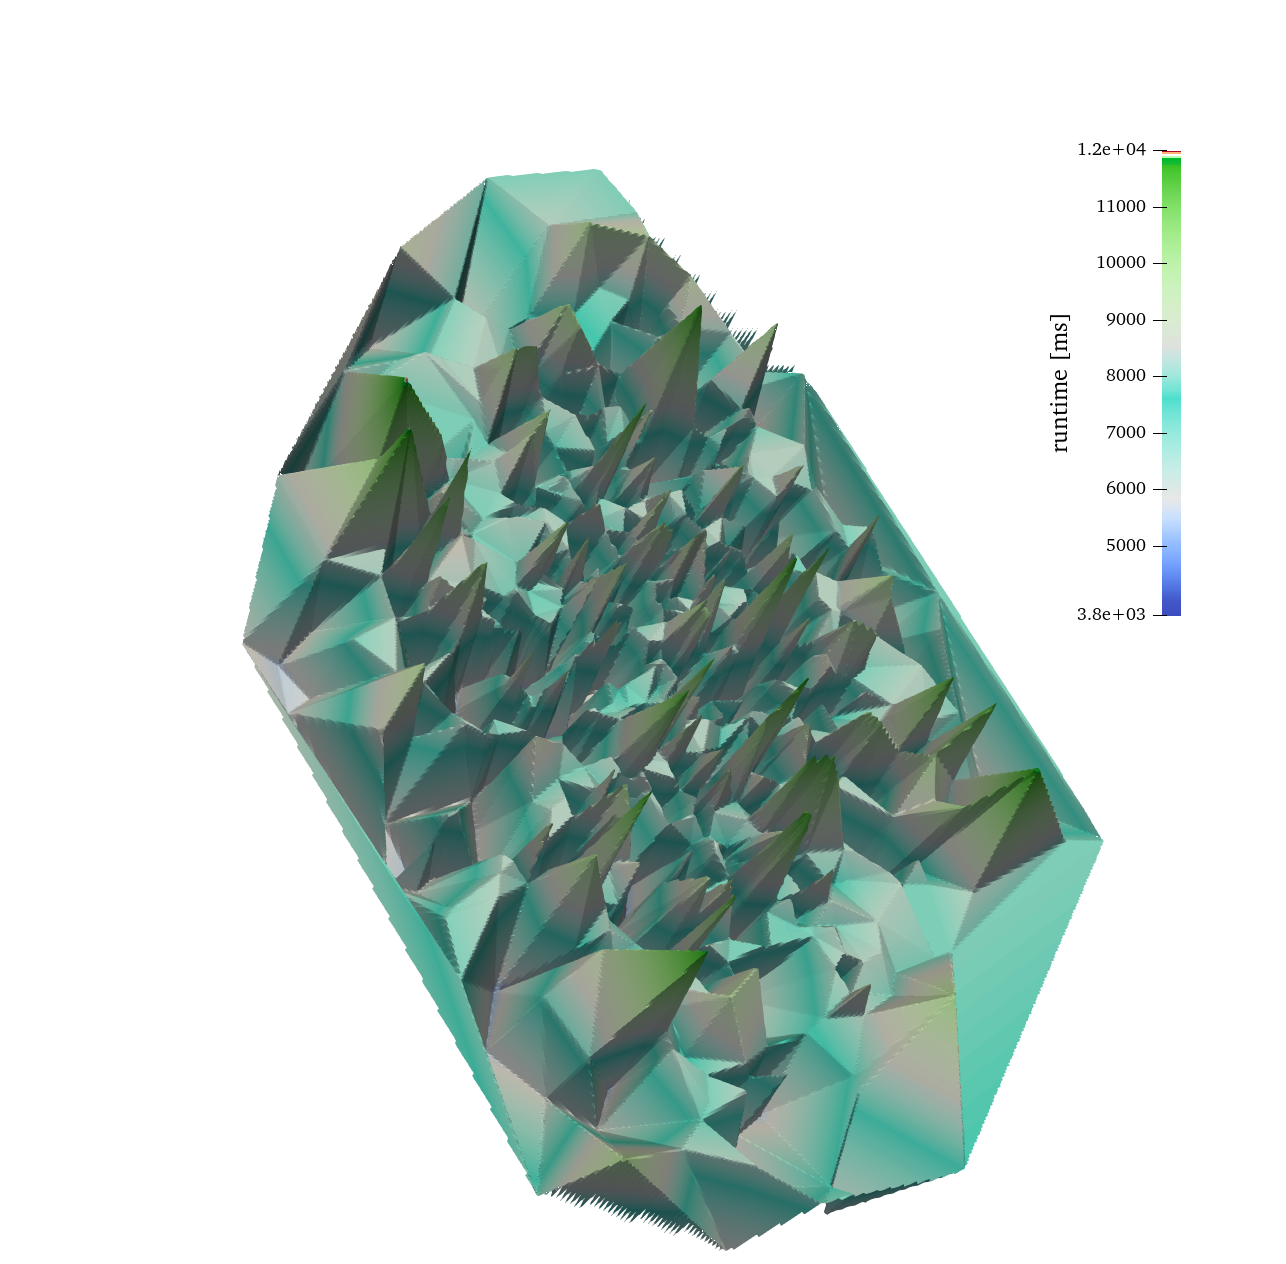
\includegraphics[width=\textwidth]{figures/coolidge-af-space3.png}
	\caption{A visualization of a random projection of the mapping space}
	\label{fig:mapping_space_visualization}
\end{figure}

Figure~\ref{fig:mapping_space_visualization} shows a rendering of the design space of mappings for the audio filter \ac{CPN} benchmark onto the MPPA3 coolidge. 
We generate this rendering using the methods of~\cite{visualloss}, which generate a smoothening from a triangulation of a random projection of $1000$ random mappings as an artistic interpretation that we can visualize with ParaView~\cite{paraview}.
This was generated from the Euclidean norm on the mapping space interpreted as vectors.
The height of the mountains and valleys in this landscape, as well as their coloring, represent the value of the execution time for the mappings being visualized.
We see how the mapping space has multiple local minima and maxima, a fact which we will discuss more in Section~\ref{sec:dse}. 

\subsection{Low-distortion Embeddings}

We have seen so far how we can endow the mapping space with multiple metrics $d_M : M \times M \rightarrow \mathbb{R}_{\geq 0}$ to define distances between mappings.
A problem with this is that the mapping space is a discrete space, with a very large cardinality.
To algorithmically do any computation in this space, e.g. in \ac{dse}, we need to iterate through the whole space.
For example we might have a mapping $m_0$, for which we want to find all mappings that are within a radius $r$ of it, i.e. compute the ball $B_r(m_0)$ with radius $r$ around $m_0$.
For this we need to iterate over all $m \in M$ and calculate if $d_M(m_0,m) \leq r$, which is intractable for all but the simplest examples.

To deal with this, we use established methods from discrete geometry to calculate \emph{low-distortion embeddings}\index{low-distortion embeddings}.
A mapping $\iota : M \hookrightarrow \mathbb{R}^n$ such that there exists a $D > 0$ with
\begin{align}\label{eqn:distortion} 1/D d(x,y) \leq \| \iota(x) - \iota(y) \| \leq d(x,y) \end{align}
is called an embedding with distortion $D$.
In other words, the \emph{relative error} of the distances is at most $D$.
We can calculate a low-distortion embedding for a finite metric space using convex optimization~\cite{matouvsek} (cf. Appendix~\ref{appendix:metric}).
This allows us to work with vectors of real numbers which make many algorithmic tasks scalable, e.g. computing random points in a ball.

Since the size of the mapping space grows exponentially with the number of tasks and changes for every application, computing such an embedding for a large mapping space every time we want to do \ac{dse} would also be intractable.
We can avoid this by using the orthogonal sum construction from Equation~\ref{eqn:orthogonal_sum}.
Given an embedding $\iota : A \hookrightarrow \mathbb{R}^k$ with distortion $D$ for the architecture with a given metric $d_A$, we can construct an embedding $\iota^k$ of the mapping space defined as in Equation~\ref{eqn:orthogonal_sum} with distortion $D$.
\begin{theorem}[Theorem III.1 of~\cite{goens_mcsoc18}]
\label{thm:iotad}
Let $\iota: (\mathcal{M}, d) \hookrightarrow (\mathbb{R}^n, \| \cdot \|_p)$ be an embedding with distortion $D$ and define $\iota^{k} : (\mathcal{M}^k,d_p) \hookrightarrow (\mathbb{R}^{nk}, \| \cdot \|_p)$ as
$\iota^k ( (x_1,\ldots,x_k)) = (\iota(x_1),\ldots,\iota(x_k))$. Then $\iota^k$ is an embedding with distortion of at most $D$.
\begin{proof}
It is clear why $\iota^k$ is an embedding (well-defined and injective), since $\iota$ is one. The distortion follows from the homogeneity of the $\| \cdot \|_p$-norm applied to Equation~\ref{eqn:distortion}.
\end{proof}
\end{theorem}
	  
The mapping space can still have a very high dimension, a problem usually called the \emph{curse of dimensionality}.\index{curse of dimensionality}
With this construction, for the metric without the extra dimensions, the dimension of the embedding $\iota^k$ is $k |V_A| = |V_K| |V_A|$.
A method to improve this is to use the Johnson-Lindenstrauss lemma to reduce the dimension with a projection.\index{Johnson-Lindenstrauss reduction}
We do this with an iterative method, described in Algorithm~\ref{algo:jl-iteration}

\begin{algorithm}
	\caption{Iterative dimensionality reduction via the Johnson-Lindenstrauss lemma.} 
	\label{algo:jl-iteration}
	\begin{algorithmic}[1]
	  \Input{A discrete metric space $M$, a low-distortion embedding $\iota : M \hookrightarrow \mathbb{R}^n$ and a target distortion $D$.}
	  \Output{An embedding with dimension $\leq n$ and distortion at most $D$.}
	 \State dim $\leftarrow$ 1
	 \While dim $\leq n$
	   \For{ $\_ \in \text{numIterationsPerDim}$}
		       \State $\tilde \iota \leftarrow \operatorname{JLReduction}(\iota,\text{dim})$
			   \State $\tilde D \leftarrow \operatorname{CalculateDistortion}(\tilde \iota)$
			   \If{$\tilde D \leq D$}
			       \Return{$\tilde \iota$}
			   \EndIf
	   \EndFor 
	   \State dim $\leftarrow 2 \text{dim}$
   \EndWhile
   \Return $\iota$
	\end{algorithmic}
\end{algorithm}

Algorithm~\ref{algo:jl-iteration} exponentially increases the dimension in a fashion akin to a binary-search, running \texttt{numIterationPerDim} iterations of a Johnson-Lindenstrauss transform and testing the distortion to see if a target distortion has been reached.
Using this algorithm, or variants thereof, we can control the trade-off between the distance and the dimension of the embedding.

We can combine these embeddings with symmetries, by first calculating a canonical representative (cf. Problem~\ref{prob:equiv} of Section~\ref{sec:symmetries}) and then calculating the embedding using $\tilde iota^k$ as defined here.
We used these methods to evaluate and compare multiple metrics. 
A useful property of this metric is if the distance between two mappings correlates with the (relative) relation of their runtimes.
In other words, we would expect a good metric to be larger for mappings that have very different performance and lower when mappings have similar performances.

To compare the different metrics and embeddings, for each of them we calculated $1000$ mappings of the audio filter benchmark on the Odroid XU4 platform. 
For a random subset of the $1000^2 = 10^6$ pairs of mappings we calculated the (relative) distance between two mappings and the relative runtime of the simulation on these two mappings.
This is what is shown in the figure for each metric and embedding combination. 

\begin{figure}[h]
	\centering
   \resizebox{1.00\textwidth}{!}{\inputTikz{metric_spaces_comparison_exynos.tex}}
	\caption{Comparison of multiple distance metrics on the Odroid XU4 platform.}
	\label{fig:metric_comparison_exynos}
\end{figure}

Figure~\ref{fig:metric_comparison_exynos} shows the comparison of the different metrics and embeddings.
In the figure, the metrics described in this section are labeled as follows: We call \texttt{SimpleVector} the Euclidean norm on the mappings described as simple vectors. 
The metric based on the latencies as motivated from Figure~\ref{fig:intuition_metric} we denote as \texttt{MetricSpaceEmedding}, whereas we add the annotation \texttt{ED} for the metric with extra dimensions which accounts for heterogeneous \acp{PE}.
The variants described as \texttt{SymmetryEmbedding} and \texttt{SymmetryEmbedding ED} are the two respective metrics combined with the symmetries, as described above. 

The results from the figure show that there is basically no correlation between mappings distance and the (relative) runtimes.
A mapping can be very far apart and have (almost) the same execution time. 
This seems very plausible if we consider the symmetries of the problem.
The symmetry reduction as used in the figure, for example did not consider the application symmetries (cf. Section~\ref{sec:symmetries}).
Moreover, some \emph{similarities}\index{mapping similarities} are also not considered.
The computation for the \ac{FFT} and \ac{IFFT} in the audio filter benchmark is virtually identical, yet not precisely identical, and would not be captured by application symmetries either.
In practice, this leads to very similar if not identical mapping execution times nevertheless.

A perhaps better assessment of the metrics is to ask what the \emph{maximal} relative execution time is possible for a given distance.
While we understand why two similar mappings which are far appart will have similar results, we would expect two mappings that are close to each other to have similar execution times with a good metric.
To test this, we take the same results of Figure~\ref{fig:metric_comparison_exynos} and just consider the maximal relative execution time for two mappings which are (at most) the given distance appart.

\begin{figure}[h]
	\centering
   \resizebox{1.00\textwidth}{!}{\inputTikz{metric_spaces_comparison_max_exynos.tex}}
	\caption{Comparison of multiple distance metrics as predictors of the \emph{maximal} run-time difference on the Odroid XU4 platform.}
	\label{fig:metric_comparison_max_exynos}
\end{figure}

Figure~\ref{fig:metric_comparison_max_exynos} shows this maximal relative execution times for the data of Figure~\ref{fig:metric_comparison_exynos}. 
It also includes a linear regression of the points for each metric and embedding.
We can see that indeed, most of the metrics are pretty good as a \emph{bound} on the relative runtime.

\begin{figure}[h]
	\centering
   \resizebox{0.95\textwidth}{!}{\inputTikz{metric_spaces_comparison_coolidge.tex}}
	\caption{Comparison of multiple distance metrics on the MPPA3 Coolidge platform.}
	\label{fig:metric_comparison_coolidge}
\end{figure}

The Odroid XU4 architecture is comparatively small, which obviously has consequences for the mapping space.
There is, for example, less problems with the curse of dimensionality and overall a smaller (discrete) space.
How does the situation change for the MPPA3 Coolidge?
Figure~\ref{fig:metric_comparison_coolidge} shows the same comparison as above for the MPPA3 Coolidge. 
We can see that the space is more complex.
In particular, the extra dimensions clearly make a difference, separating the space into more discrete distinct points, with clearly visible vertical lines.
We will discuss these vertical lines further in Section~\ref{sec:dse}.

\begin{figure}[h]
	\centering
   \resizebox{0.95\textwidth}{!}{\inputTikz{metric_spaces_comparison_max_coolidge.tex}}
	\caption{Comparison of multiple distance metrics as predictors of the \emph{maximal} run-time difference on the MPPA3 Coolidge platform.}
	\label{fig:metric_comparison_max_coolidge}
\end{figure}

Similar to the case for the Odroid XU4, Figure~\ref{fig:metric_comparison_max_coolidge} shows the same comparison with the maximal run-time difference for the MPPA3 Coolidge.
Again we see that many metrics seem to be a decent bound for the difference in execution time, although less so than for the simple Odroid XU4 paltform.
The Euclidean norm on the simple vector mappings, for example, is considerably worse than in this case than in the Odroid XU4.
We can quantify more precisely how good metrics are as a bound for the execution time by comparing the $R^2$ value as goodness of fit assessment of the depicted linear regressions.

\begin{figure}[h]
	\centering
   \resizebox{0.75\textwidth}{!}{\input{generated/metrics_regression_rsq.tex}}
	\caption{Comparison of the predictive power of multiple distance metrics.}
	\label{fig:metric_regression}
\end{figure}

Figure~\ref{fig:metric_regression} shows the $R^2$ value, comparing the predictive power of the different distance metrics and their embeddings.
Here it is also very clear that the Euclidean norm on simple vectors is not so good for the MPPA3 Cooldige, while it is comparable to other metrics in the Odroid XU4.
We also see how the curse of dimensionality yields a trade-off not only in the computation time (for larger-dimensional spaces), but also in the predictive quality of the different norms.
This is more visible on the MPPA3 Coolidge.